% Method-centered visual draft. Schematics have editable diagrams.net XML.
\documentclass[letterpaper,journal]{IEEEtran}
\usepackage{amsmath,amssymb,graphicx,booktabs,cite,url,capt-of}
\usepackage{algorithm,algpseudocode,array}
\newcolumntype{P}[1]{>{\raggedright\arraybackslash}p{#1}}
\usepackage{flafter}
\usepackage[hidelinks]{hyperref}
\begin{document}
\title{Adapting a Pretrained Vision-Language-Action Model to a New Robot Embodiment without Human Demonstrations through Staged Reinforcement Learning}
\author{}
\IEEEaftertitletext{\begin{minipage}{\textwidth}
\centering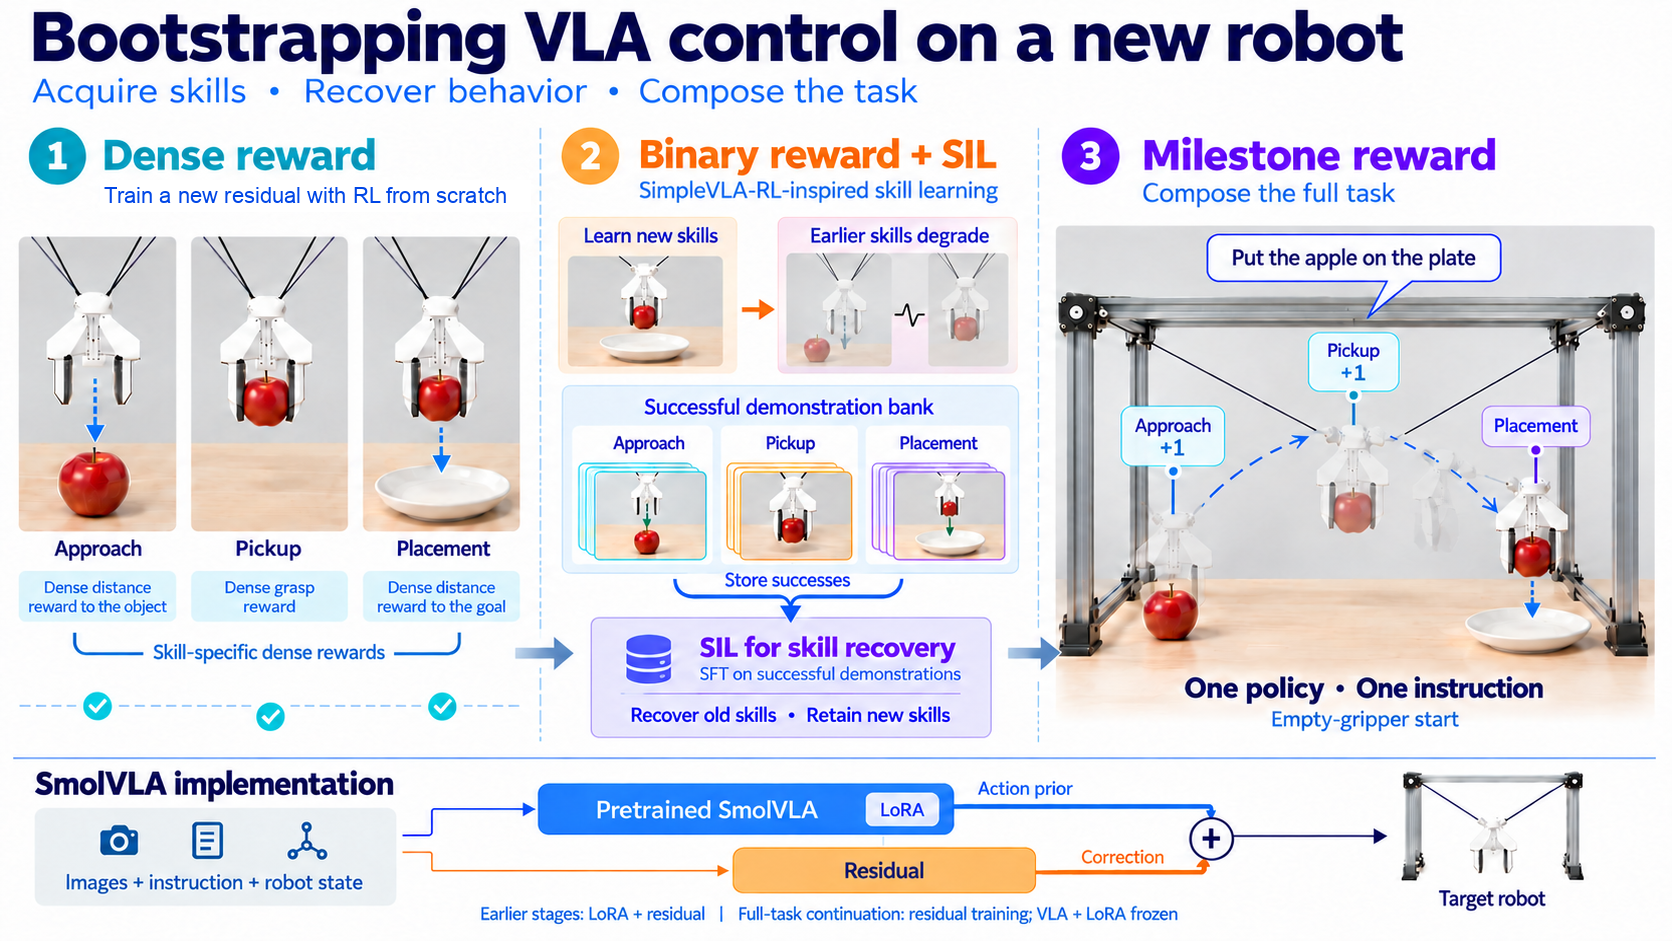
\includegraphics[width=\textwidth]{figures/abstract_overview.png}
\captionof{figure}{Proposed pipeline and SmolVLA implementation. A newly initialized residual controller is trained over the retained pretrained SmolVLA expert; ``from scratch'' refers to this residual only. Dense feedback acquires skills; binary refinement and balanced self-imitation consolidate them; milestone-based RL learns the complete task under one instruction. Skill-specific resets are used during acquisition. Full-task evaluation starts with an empty gripper and uses no external switching between specialists.}
\label{fig:hero}
\end{minipage}
\vspace{1em}}
\maketitle
\begin{center}\small\textbf{WORKING DRAFT --- 29 October 2026}\end{center}
\begin{abstract}
Adapting a pretrained vision-language-action (VLA) model to a new robot usually requires demonstrations collected on that robot. We investigate adaptation without collecting human demonstrations for the target embodiment. A newly initialized residual controller, placed over a retained pretrained SmolVLA action expert, first acquires approach, pickup, and placement skills through reinforcement learning (RL) with dense rewards. Binary refinement and instruction-balanced self-imitation then consolidate these skills, and milestone-based RL trains one policy for the complete instruction from an empty-gripper start. Supervised stages use only automatically generated data: successful policy rollouts, a scripted simulator oracle, and policy rollouts with scripted controller assistance. On a simulated cable-driven parallel robot (CDPR), the resulting controller completes 723 of 1,024 full pick-and-place attempts (70.61\%) under a strict success criterion on a development validation panel. In an auxiliary LIBERO-Spatial study with OpenVLA-OFT, our terminal-only implementation moves a 61.0\% initial policy to 61.7\% after 160 updates, and dense-plus-phase reward reaches 65.3\%; these single-run intervals overlap. The results establish feasibility of the schedule in simulation. They do not isolate the contribution of individual stages.
\end{abstract}

\begin{IEEEkeywords}
Robot learning, reinforcement learning, manipulation, vision-language-action models, robot adaptation.
\end{IEEEkeywords}
\section{Introduction}\label{sec:introduction}
Vision-language-action (VLA) models are usually adapted to a new robot by supervised fine-tuning on demonstrations collected with that robot. SmolVLA, for example, fine-tunes on 50 demonstrations per real-world task~\cite{smolvla}. iRe-VLA begins its real-robot experiments with 2,000 teleoperated trajectories~\cite{irevla}, and PLD fine-tunes its base policy on 200 teleoperated trajectories before residual RL~\cite{pld}. Each new embodiment needs a teleoperation interface, operator time, and a fresh collection campaign. We investigate whether this collection step can be avoided by making reinforcement learning (RL) the first stage of target-embodiment adaptation.

RL from a pretrained VLA on a new action interface faces three obstacles. The initial policy rarely completes a multi-stage task, so binary success provides little guidance. Training component skills separately helps exploration, but later skills can erase earlier ones. Finally, the retained skills must be composed into one behavior for the complete instruction. Consider \emph{put the apple on the plate}. A failed rollout may contain a correct approach and grasp followed by a poor release, and treating the entire attempt as a failure discards that distinction.

We address these obstacles with the schedule in Fig.~\ref{fig:hero}. A newly initialized residual controller is placed over a retained pretrained SmolVLA action expert~\cite{smolvla}. It first acquires approach, pickup, and placement skills through RL with dense rewards. Binary refinement then targets skill completion, and instruction-balanced self-imitation retains successful behavior across instructions. Finally, milestone-based RL trains the same policy to execute the complete instruction from an empty-gripper start.

The data requirement is precise. We collect no human demonstrations on the target robot. Supervised stages fit only automatically generated trajectories: successful policy rollouts, a scripted simulator oracle, and policy rollouts with scripted controller assistance (Section~\ref{sec:lineage}). These trajectories are demonstrations, so the setting is not demonstration-free; it removes human collection. Simulator construction, reward and reset design, oracle engineering, and RL compute remain. We therefore make no claim of lower total adaptation cost.

This paper extends our earlier preprint, which adapted OpenVLA-OFT to the same cable-driven parallel robot (CDPR) with RL alone and reported directional motion and object reaching, with 9.75\% strict success on \emph{move to \textless object\textgreater}~\cite{nurtdinov2026rlboot}. Here we address complete pick-and-place, skill consolidation, and a different controller, a residual over SmolVLA. A separate study on LIBERO-Spatial with OpenVLA-OFT~\cite{openvlaoft,libero} examines intermediate feedback for full-task RL. It does not evaluate the full schedule.

Our contributions are:
\begin{enumerate}
\item A staged adaptation method for a pretrained VLA on a new robot without target-embodiment human demonstrations: dense-reward skill acquisition by a new residual controller, binary refinement with instruction-balanced self-imitation, and milestone-based learning of the complete instruction.
\item A milestone credit rule that retains local credit for achieved approach and pickup when later placement fails.
\item An empirical instantiation on a simulated CDPR, with a full training-lineage account, a skill-by-stage record, and strict full-task evaluation; and an auxiliary LIBERO-Spatial comparison of intermediate feedback.
\end{enumerate}

\section{Related Work}\label{sec:related}
\textbf{Group-relative RL and dynamic sampling.} GRPO estimates policy advantages by comparing returns within groups of sampled trajectories~\cite{deepseekmath}. DAPO filters groups with uniform binary outcomes and collects additional samples to keep the training batch informative~\cite{dapo}. SimpleVLA-RL adapts group-relative optimization to interactive VLA rollouts~\cite{simplevlarl}. It starts from a supervised OpenVLA-OFT checkpoint trained on LIBERO demonstrations, either all of them or one per task. We use DAPO-style group filtering and resampling during skill learning.

\textbf{RL with supervised consolidation.} iRe-VLA alternates RL on the action head, with a frozen vision-language backbone, and supervised updates on expert data together with successful online trajectories~\cite{irevla}. Probe, Learn, Distill (PLD) trains residual actors over a frozen VLA, seeds their buffers with successful base-policy rollouts, and distills hybrid trajectories into the generalist~\cite{pld}. Our self-imitation step similarly fits successful experience. Its instruction-balanced bank retains earlier skills during sequential training. We adopt PLD's residual principle for the new action interface.

\textbf{Adaptation data.} Table~\ref{tab:related} compares close methods by the data they need on the target robot. iRe-VLA and PLD begin from policies fine-tuned on human target-robot demonstrations. ET-VLA reduces the need for real demonstrations through synthetic continued pretraining, then fine-tunes on target-embodiment data~\cite{etvla}. Our earlier preprint used RL alone on the CDPR, but stopped at reaching~\cite{nurtdinov2026rlboot}. The present work keeps the no-human-demonstration setting and reaches complete pick-and-place. However, it uses automatically generated supervised data, which the preprint did not.

\begin{table*}[!t]
\caption{Data and training attributes of close methods, from the cited papers. ``n.s.'': not stated in the source. ``Before RL'' is target-task competence at the start of RL.}
\label{tab:related}\centering\footnotesize
\setlength{\tabcolsep}{3pt}
\begin{tabular}{@{}lP{3.0cm}P{3.1cm}P{2.0cm}P{2.5cm}P{1.6cm}P{1.4cm}@{}}\toprule
Method & Human target demos & Other adaptation data & Before RL & RL-trained module & Embodiment change & Full-task eval.\\\midrule
iRe-VLA~\cite{irevla} & 50/task (MetaWorld); 2,000 (Panda) & Online successes & SFT policy & Action head; VLM frozen & n.s. & Yes\\
PLD~\cite{pld} & Benchmark SFT (n.s.); 200 ($\pi_0$, real) & Base-policy successes; hybrid rollouts & SFT policy & Residual; base frozen & n.s. & Yes\\
SimpleVLA-RL~\cite{simplevlarl} & 1/task or full LIBERO set & --- & 63.6\% (1 demo, Spatial) & Full parameters & No & Yes\\
ET-VLA~\cite{etvla} & Target-embodiment fine-tuning data & Synthetic continued pretraining & --- (SFT) & --- & Yes (bimanual) & Yes\\
RL bootstrapping~\cite{nurtdinov2026rlboot} & 0 & --- & n.s. & OpenVLA-OFT (PPO, GRPO) & Yes (CDPR) & Reaching only\\
Ours & 0 & Policy successes; scripted oracle; controller-assisted rollouts & 2.6\%$^\dagger$ & Residual; LoRA in SFT & Yes (CDPR) & Yes\\\bottomrule
\end{tabular}\\[2pt]
\footnotesize$^\dagger$Strict full-task success at the start of milestone RL, after the inherited supervised seeding stages (Table~\ref{tab:lineage}).
\end{table*}

\section{Methods}\label{sec:method}
The goal is to adapt a pretrained VLA to complete language-conditioned manipulation tasks on a target robot without collecting human demonstrations on that robot. We study multi-stage pick-and-place tasks: an instruction such as \emph{put the apple on the plate} requires approach, grasp, lift, transport, and release. The policy receives camera images, proprioception, and an instruction, predicts an action chunk, and executes a prefix before observing again. We evaluate complete-task success independently of the reward used for training.

\textbf{Target embodiment.} The CDPR suspends its end effector from four cables. Each cable runs from a fixed anchor to a position-controlled slider. The tool adds a yaw joint and a two-finger gripper. Each executed action is a normalized five-dimensional increment: Cartesian translation (up to 1.5\,cm per axis), yaw (up to 0.08\,rad), and gripper opening. A fixed inverse-kinematics controller converts the end-effector target to cable lengths. The policy therefore learns the mapping from images and language to Cartesian increments, while cable actuation remains hand-built. Observations are an overview and a wrist camera together with six proprioceptive values. SmolVLA was pretrained on 481 community datasets, which its authors describe as collected from a single robot type, the SO100 serial arm~\cite{smolvla}. A cable-driven parallel mechanism and this action interface are absent from that documented robotic data. We make no claim about images in its vision-language pretraining.

\textbf{Data contract.} We distinguish human demonstrations on the target robot (none are used), automatically generated trajectories used as supervised action targets, and assistance used only to choose starting states. Pretrained robot data enter only through the SmolVLA weights. Section~\ref{sec:lineage} reports each category for every ancestor of the evaluated controller.

Skills are acquired with their own instructions, success conditions, and starting states, whereas composition and evaluation start with an empty gripper and one complete-task instruction.


\subsection{Dense Acquisition, Binary Refinement, and Self-Imitation}\label{sec:skill_acquisition}
We use dense rewards only at the beginning of adaptation to learn a base policy for simple skills. Each skill has a distinct instruction and reset distribution:
\begin{itemize}
\item \textbf{Approach:} \emph{move to \textless object\textgreater}. Reach the named object with an empty gripper, without requiring a grasp.
\item \textbf{Pickup:} \emph{pick up \textless object\textgreater}. Learn to grasp and lift the named object.
\item \textbf{Placement:} \emph{put \textless object\textgreater\ into bowl} or \emph{put \textless object\textgreater\ on the plate}. Start with the object already grasped and learn transport and release at the named destination.
\end{itemize}
The object placeholder is replaced by its name. These instructions condition the policy on the requested skill and target; the instruction remains attached to each retained trajectory. Distance reduction and manipulation events guide initial acquisition. We then refine the skills with binary success rewards and consolidate them through self-imitation.

Successful trajectories are retained by instruction. When later training degrades earlier skills, self-imitation fits a balanced mixture of earlier and current successes:
\begin{equation}
\mathcal L_{\rm SI}=\mathbb E_{\rm success}
\left[\|\hat a-a\|^2\right].
\label{eq:si_loss}
\end{equation}
Here $\hat a$ is the predicted action and $a$ is the recorded executed action. The average balances instructions and excludes unused action slots. Policy-dependent features are refreshed before fitting. Balancing is intended to keep the newest skill from dominating the fit. We have not compared it with unbalanced replay.

Full-task success requires each stage in turn, so its probability is the product of conditional stage success rates. Low but nonzero stage rates therefore permit occasional complete successes, which milestone credit can then reinforce. We treat skill-success targets as practical transition criteria, not necessary conditions. Isolated skill tests also differ from the full task in prompt and start distribution.

Algorithm~\ref{alg:paper_pipeline} summarizes the schedule. Progress is checked with fixed skill evaluations. After an initial training period, automated stages can end at a success target or a plateau; budget exhaustion also ends a stage. The CDPR sequence used validation-guided manual transitions. After consolidation, all learned skills are evaluated again. Automated runs retain the consolidation update only when recovery improves the degraded skills on average and keeps other skills within tolerance.

When the consolidated policy has no measurable full-task success, the schedule allows an optional seeding stage that fits $\mathcal L_{\rm SI}$ to automatically generated full-task trajectories. The CDPR lineage used two such stages, described in Section~\ref{sec:lineage}: scripted-oracle demonstrations, and chains of earlier learned skill policies with scripted controller assistance.
% Method-level schedule. Automatic stopping is implemented for WX200;
% the historical CDPR sequence used validation-guided manual transitions.
% The optional seeding stage reflects the CDPR lineage (evidence/DATA_LINEAGE_AUDIT_20261029.md).
\begin{algorithm}[!t]
\caption{Staged VLA adaptation}
\label{alg:paper_pipeline}
\small
\begin{algorithmic}[1]
\Require Pretrained VLA, simple-skill instructions, fixed evaluations
\State Load the pretrained VLA; initialize a new residual controller and success banks
\For{reward mode: dense acquisition, then binary refinement}
    \For{skill: approach, pickup, placement}
        \Repeat
            \State Collect same-scene rollout groups for the skill
            \State Update with $\mathcal L_{\rm RL}$; retain successful trajectories
            \State Evaluate skill success
        \Until{target, plateau, or stage budget ends training}
        \State Evaluate retention of all learned skills
        \If{earlier skills have degraded}
            \State Balance earlier and current successful experience
            \State Fit $\mathcal L_{\rm SI}$; validate recovery and retention
        \EndIf
    \EndFor
\EndFor
\If{full-task success is not measurable}
    \State Optional seeding: fit $\mathcal L_{\rm SI}$ to automatically generated
    \Statex \hspace{\algorithmicindent}full-task trajectories (oracle or assisted chains)
\EndIf
\State Initialize full-task learning from the consolidated base policy
\Repeat
    \State Collect full-task rollouts from empty-gripper starts
    \State Assign milestone credit; protect achieved prefix skills
    \State Update with $\mathcal L_{\rm RL}$; evaluate complete-task success
\Until{target, plateau, or full-task budget ends training}
\If{composition plateaus and budget remains}
    \State Freeze VLA/LoRA; retain the bounded residual
    \State Reset optimizer; keep milestone rewards unchanged
    \Repeat
        \State Collect full-task groups; execute clipped commands
        \State Store pre-clipping samples and episode offsets
        \State Score samples conditional on their stored offsets
        \State Assign milestone credit; protect achieved prefix skills
        \State Update residual and exploration with $\mathcal L_{\rm RL}$
        \State Evaluate complete-task success
    \Until{target, renewed plateau, or budget exhaustion}
\EndIf
\State \Return One policy for the complete instruction
\end{algorithmic}
\end{algorithm}


\subsection{SmolVLA with a Newly Initialized Residual}\label{sec:architecture}
\begin{figure*}[!t]
\centering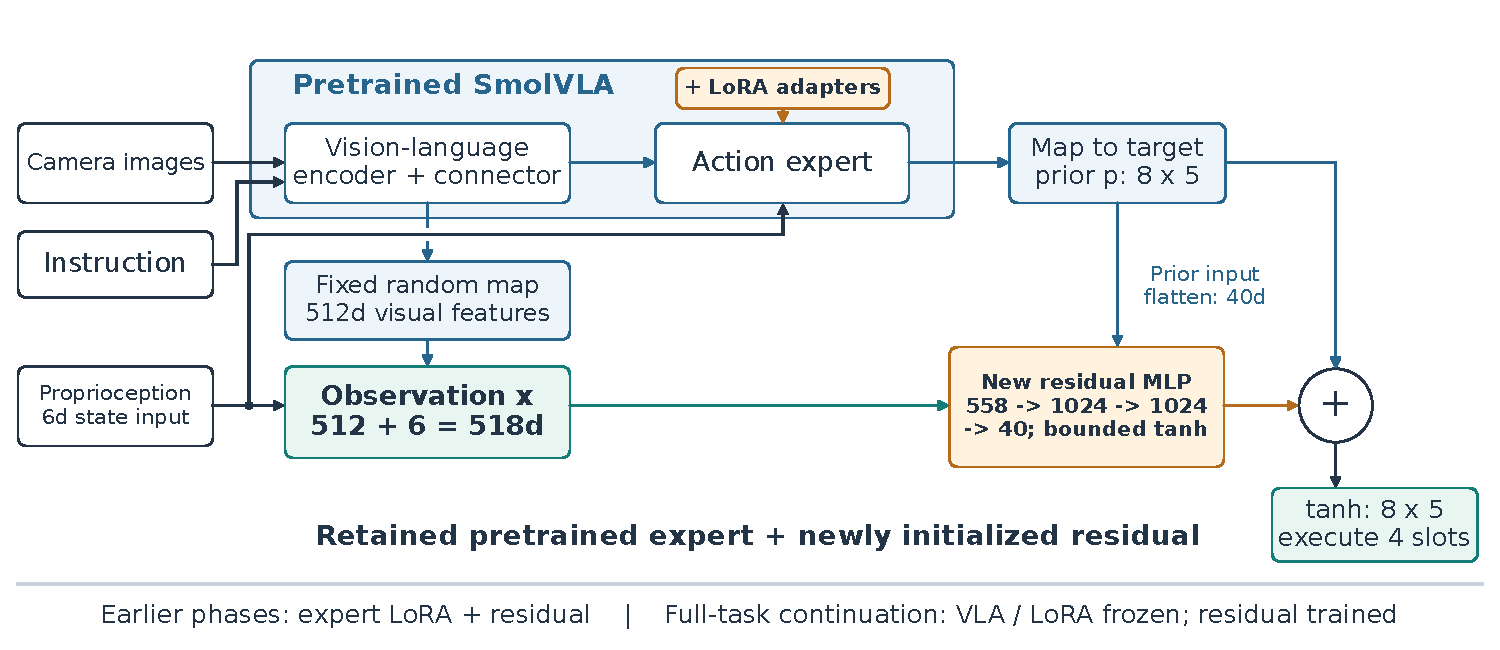
\includegraphics[width=\textwidth]{figures/smolvla_residual_lora.pdf}
\caption{SmolVLA implementation. The pretrained VLM and action expert are retained and frozen. A newly initialized residual combines 518 observation features with a 40-dimensional action prior. LoRA adapts the expert in supervised stages; the evaluated full-task continuation freezes the VLA and LoRA weights. Feature and action dimensions refer to the five-channel controller.}
\label{fig:architecture}
\end{figure*}

Figure~\ref{fig:architecture} and Table~\ref{tab:modules} describe the evaluated controller. The SmolVLA vision-language model and action expert are loaded from pretrained weights and are never reset or directly trained. Their action chunk is mapped to the five target channels; eight action slots form a 40-dimensional prior. Following the residual principle of PLD~\cite{pld}, a residual MLP is created with default initialization at the start of adaptation and is the component trained from scratch. It receives a 518-dimensional observation and the prior, and predicts a bounded correction; the combined action is bounded before execution. The observation consists of six proprioceptive values and a 512-dimensional visual feature. This feature is a fixed random projection of SmolVLA's connector tokens from both cameras. It is neither pretrained nor learned.

LoRA adapters on the action expert start with zero contribution. They are updated only in supervised stages, including the seeding stage, and are frozen during all full-task RL. During full-task training, only the residual and the exploration parameters change. The backbone, action mapping, and feature dimensions can change with the embodiment; the training schedule remains the same.

\begin{table}[!t]
\caption{Modules of the evaluated controller.}
\label{tab:modules}\centering\footnotesize
\setlength{\tabcolsep}{3pt}
\begin{tabular}{@{}lllr@{}}\toprule
Module & Initialization & Trained & Params\\\midrule
SmolVLA VLM & Pretrained & Never & $\approx$350M$^a$\\
SmolVLA action expert & Pretrained, not reset & Never & $\approx$100M$^a$\\
Expert LoRA (r\,=\,16, $\alpha$\,=\,32) & Zero update & SFT stages & 3.42M\\
Visual projection & Fixed random & Never & ---$^b$\\
Residual MLP & New (default) & All stages & 1.66M\\
Exploration $\log\sigma$ & Constant $-1.2$ & RL stages & 40\\\bottomrule
\end{tabular}\\[2pt]
\raggedright\footnotesize$^a$As documented for the 450M SmolVLA~\cite{smolvla}. $^b$Fixed $30{,}720\times512$ map.
\end{table}

\subsection{Milestone-Based Full-Task Composition}\label{sec:composition}
After skill consolidation, the base policy learns the complete task from empty-gripper starts using binary milestone rewards. The full-task prompt is \emph{put \textless object\textgreater\ into \textless destination\textgreater}, where the destination is plate or bowl. This includes the plate wording \emph{into plate}, whereas the isolated plate-placement skill uses \emph{on the plate}. The full-task instruction stays fixed throughout approach, pickup, and placement. Continuous dense shaping is confined to the initial simple-skill acquisition in Section~\ref{sec:skill_acquisition}. The LIBERO reward comparison examines how intermediate feedback can support execution of a complete instruction.

\label{sec:dense_method}
We consider terminal-only, phase-only, and combined dense-and-phase rewards. The combined reward uses a manually defined sequence of reach, grasp, lift, move, and place phases, with a hand-specified progress function for each phase.

At each simulator step, the tracker uses object and gripper state to compute progress for the active phase. Reaching progress increases as gripper--object distance decreases; grasping combines proximity with gripper closure and grasp state; lifting uses height gained above the initial object position; transport uses planar object--target distance; placement uses target proximity, release, and environment success. Each progress measure is normalized to the interval from zero to one. For progress $p_t$ and the phase's previous maximum $p_{\rm best}$, the rewarded increment is $\max(p_t-p_{\rm best},0)$. A completion predicate advances the tracker to the next phase and produces a phase bonus. The weighted progress increment and phase bonus are bounded and combined with terminal feedback. The native task-success verifier remains unchanged.

In the phase-only condition, the continuous progress weight is zero, leaving phase-completion bonuses and terminal feedback.

This construction needs a progress function, normalization, and state variables for every phase of each new task. Our adaptation pipeline therefore uses dense feedback only for simple skills, and full-task training uses binary milestones defined by completion predicates.

The motivation follows from a simple group calculation. For $G$ independent rollouts from one scene, each with success probability $p$, the probability of observing both success and failure is
\begin{equation}
P_{\rm mixed}=1-p^G-(1-p)^G.
\label{eq:mixed}
\end{equation}
With eight rollouts, this probability is only 21.6\% at 3\% success, but 94.2\% at 30\% success. Milestones can therefore provide informative comparisons before complete-task success becomes common.


Three ordered, irreversible milestones are defined by predicates on the simulator state. Approach ($M_1$) requires entering a 3\,cm neighborhood of the grasp point with the gripper open and the object undisplaced. Pickup ($M_2$) requires a persistent physical grasp and a lift of at least 5\,cm while held. Placement ($M_3$) requires the strict destination contract: correct receptacle, intentional release, settled geometry, and no carry slip or wrong placement. Each milestone pays $+1$ once.

The rule is simple: a later placement failure should not remove local credit for a successful approach or pickup. Actions up to the one that triggers $M_1$ form the approach segment, actions up to $M_2$ form the pickup segment, and later actions form the placement segment. Each segment receives its own group-relative advantage, computed among the eight rollouts of the same scene. Groups without variation in a segment are dropped from that segment, and the three segment losses receive equal weight. Full-task completion adds a bonus of 1 to the return. A negative completion advantage is suppressed on segments whose milestone was achieved. The policy still executes the complete instruction without an external controller switching between specialists.

\subsection{Stabilized Updates and Full-Task Continuation}\label{sec:rl_loss}
We use a clipped group-relative policy loss with entropy regularization:
\begin{equation}
\mathcal L_{\rm RL}=\mathcal L_{\rm clip}-\eta\mathcal H.
\label{eq:rl_loss}
\end{equation}
$\mathcal L_{\rm clip}$ is the PPO surrogate on the likelihood ratio of each rollout's actions, with the group-normalized advantage of its segment. It uses separate lower and upper clipping bounds, 0.20 and 0.28. The entropy term $\mathcal H$, weighted by $\eta=2\times10^{-4}$, maintains exploration during manipulation and composition. Together, these choices keep early updates conservative while successful behavior is still rare.

During skill learning, DAPO-style dynamic sampling filters uninformative groups and collects additional rollout groups within the configured collection budget~\cite{dapo}. With binary rewards, uniform outcomes provide no group-relative contrast. During dense acquisition, filtering instead checks within-group return variation, so partial progress can provide a learning signal before a group contains a successful skill execution.

During full-task continuation, the inherited VLA and LoRA remain frozen while the residual and exploration scale are trained with a fresh optimizer and the same milestone rewards. The controller adds Gaussian exploration noise and an episode-level offset to its predicted mean before clipping the command for execution. The offset is sampled once per episode and applied during selected phases. We store the original sample and the applied offset, then use both to evaluate its likelihood under the old and new policies~\cite{capg}.

Let $\mu_{\theta,t}$ denote the controller's predicted mean, $\sigma_\theta$ the learned exploration scale, and $b_t$ the applied offset. The sampled command $u_t$ and executed action $a_t$ are
\begin{equation}
\begin{aligned}
u_t&\sim\mathcal N(\mu_{\theta,t}+b_t,\operatorname{diag}(\sigma_\theta^2)),\\
a_t&=\operatorname{clip}(u_t,-1,1).
\end{aligned}
\label{eq:latent_action}
\end{equation}
The likelihood ratio scores the stored $u_t$ conditional on the same $b_t$. Section~\ref{sec:cdpr_results} reports complete-task performance.

\section{Experiments}\label{sec:experiments}
We first account for the training lineage of the evaluated CDPR controller and the skills measured along it. We then report skill retention during base-policy learning, the auxiliary LIBERO-Spatial feedback study, and complete-task CDPR adaptation. A WX200 evaluation is ongoing.

The CDPR simulation uses MuJoCo Warp/MJ-Lab, four object categories (apple, orange, potato, and tomato), and plate or bowl destinations. Full-task stages use 8-action chunks with a 4-action executed prefix, groups of 8 rollouts per scene, a 128-decision horizon, and 512 parallel worlds per GPU on two A40 GPUs. The continuation S11 uses a fresh Adam optimizer, learning rate $10^{-5}$, one PPO epoch per update, and initial $\log\sigma=-1.2$; its last 20M actions took 95.3\,h. Rewards, milestones, and training-only assistance read simulator state. The evaluated policy observes only the two camera images, proprioception, and the instruction.


\subsection{Training Lineage and Data Origin}\label{sec:lineage}
Table~\ref{tab:lineage} traces the evaluated controller from the pretrained model. Approach, pickup, and placement were acquired by RL with dense rewards (S1--S3), and retention cycles consolidated them by self-imitation on the policy's own successes (S4). No consolidated policy completed the full task, so two supervised stages seeded composition. S5--S6 fitted a scripted simulator oracle's pick-and-place trajectories. The oracle sets only the executed actions; observations, priors, resets, and predicates are the trainer's own. S9 fitted chains of earlier learned skill policies whose execution was assisted by scripted yaw, gripper-hold, and descent controllers, with every chain relabelled to the final instruction. Milestone RL then trained the policy without assistance (S10--S11).

Thus no human demonstrations or interventions on the CDPR enter the lineage, but automatically generated demonstrations do. The full-task result is not evidence for adaptation from the learner's own RL trajectories alone. Across S10--S11, full-task training consumed about 116M selected environment actions. Earlier stages and the oracle and chain collection add more, and some of their budgets were not retained. The unadapted model, pretrained SmolVLA with a fresh residual, was not evaluated under the full-task protocol. The earliest strict full-task measurement is 2.6\% at the start of S10, after both seeding stages.
% Source: evidence/DATA_LINEAGE_AUDIT_20261029.md. Interactions are selected
% environment actions where reported; n.r. = not reported in local evidence.
\begin{table*}[!t]
\caption{Training lineage of the evaluated CDPR controller, from the pretrained model (top) to the reported endpoint (bottom). No stage used human demonstrations or interventions on the target robot.}
\label{tab:lineage}\centering\footnotesize
\setlength{\tabcolsep}{3pt}
\begin{tabular}{@{}P{3.1cm}P{1.1cm}P{3.6cm}P{4.3cm}P{3.2cm}r@{}}\toprule
Stage & Parent & Objective & Supervised action targets & Training-only assistance & Interactions\\\midrule
S0 SmolVLA + new residual & --- & Pretrained VLA; residual default init. & --- (SO100 pretraining only) & --- & ---\\
S1 Approach & S0 & RL, dense distance reward & --- & Distance curriculum & 5.0M\\
S2 Pickup & S1 & RL, dense & --- & Gripper aligned above object & n.r.\\
S3 Placement & S1/S2$^*$ & RL, dense & --- & Object already held & 15M\\
S4 Retention cycles 1--3 & S3 & Family RL alternated with $\mathcal L_{\rm SI}$ & Own successful rollouts & Held/aligned starts in bank & n.r.\\
S5 Composition seed & S4 & $\mathcal L_{\rm SI}$ (residual) & Own successes + \textbf{scripted-oracle} pick-and-place & Oracle drives the robot & SFT only\\
S6 Re-harvested seed & S5 & $\mathcal L_{\rm SI}$ (residual) & As S5, larger oracle slice & As S5 & SFT only\\
S7 Joint sparse RL & S6 & RL, one binary reward, four instructions & --- & Mixed held/desk starts & 2.0M\\
S8 Release-recovery RL & S7 & RL, binary & --- & Gripper aligned above object & 2.1M\\
S9 Three-stage seed & S8 & $\mathcal L_{\rm SI}$ (residual, then expert LoRA) & Earlier policies chained with \textbf{scripted controller assistance}, relabelled & Handoffs between policies & SFT only\\
S10 Milestone RL & S9 & Milestone RL, residual only & --- & None (empty start, final prompt) & 56.1M\\
S11 Continuation & S10 & Milestone RL, offset-conditioned likelihood & --- & None & 60.0M\\\bottomrule
\end{tabular}\\[2pt]
\raggedright\footnotesize Interactions are selected environment actions; n.r.: not reported in the retained records. $^*$Exact parent not reconstructed. Oracle and assisted-chain collection budgets are not included.
\end{table*}

% Source: CDPR_CONSOLIDATED_PROGRESS_REPORT.md, "Instruction success by phase and
% retention cycle" and ledger entries; stage labels follow tables/lineage.tex.
\begin{table*}[!t]
\caption{Skill success by stage, in percent, with successes/attempts where recorded. Rows use different protocols (column P) and must not be read as one learning curve. ---: not measured, not zero.}
\label{tab:skill_matrix}\centering\scriptsize
\setlength{\tabcolsep}{2.5pt}
\begin{tabular}{@{}llcccccc@{}}\toprule
Stage & P & Reach & Pickup & Plate, held & Bowl, held & Plate, full task & Bowl, full task\\\midrule
S1 approach reference & D & 63.0 (645/1024) & --- & --- & --- & --- & ---\\
S2 pickup reference & D & --- & 26.0 & --- & --- & --- & ---\\
S3 placement, 15M & D & --- & --- & 71.0 & 32.0 & --- & ---\\
S4 before cycle 1 & B & 8.0 & --- & 50.0 & 23.1 & --- & ---\\
S4 after cycle 1 & B & 31.1 & --- & 52.3 & 27.7 & --- & ---\\
S4 after cycle 2 & B & 43.2 & 17.4 & 34.6 & 17.0 & --- & ---\\
S4 after cycle 3 & B & 47.8 (734/1536) & 11.9 (183/1536) & 73.8 (632/856) & 53.5 (364/680) & 0.5 (10/2168)$^\dagger$ & 1.1 (22/1928)$^\dagger$\\
S5 composition seed & B & 48.0 (737/1536) & 14.9 (229/1536) & 71.5 (612/856) & 47.9 (326/680) & 9.3 (80/856)$^\dagger$ & 2.6 (18/680)$^\dagger$\\
S7 joint sparse RL & B & 42.0 (168/400) & 14.7 (225/1536) & --- & --- & 50.0 (228/456)$^\dagger$ & 21.6 (76/352)$^\dagger$\\\midrule
S10 start (after S9) & V & --- & --- & --- & --- & 1.4 (7/512) & 3.9 (20/512)\\
S10, best separate eval. & E & --- & --- & --- & --- & 37.4 (46/123) & 33.8 (45/133)\\
S11 endpoint & V & --- & --- & --- & --- & 76.8 (393/512) & 64.5 (330/512)\\\bottomrule
\end{tabular}\\[2pt]
\raggedright\footnotesize P: D, dedicated skill reference; B, bank-harvest evaluation at registered caps; V, in-run strict full-task validation panel; E, separate strict evaluation on 256 distinct scenes. Full-task entries below the rule use an empty-gripper start and the strict criterion. $^\dagger$Earlier composed protocol: object on the desk 0.06--0.10\,m from the receptacle, scored by the earlier composed predicate. This differs from the strict full task.
\end{table*}


Table~\ref{tab:skill_matrix} records skill success along the lineage. Every component skill was measured above zero before full-task RL, and the same policy later executed the complete task. The rows use different instructions, resets, and success predicates; they document development and retention, not a single learning curve. They also do not show that instruction balancing improved later composition, which would require a control trained without it.

\subsection{Base-Policy Skill Learning and Retention}\label{sec:skill_retention}
These measurements concern dense-reward training of simple CDPR skills and their consolidation into a base policy (S1--S4), before full-task composition. Each skill uses the instruction and reset protocol in Section~\ref{sec:skill_acquisition}; placement tests start with the object already held. Learning a new skill can degrade previously learned behavior, which full-task execution later needs.

In a forgetting evaluation, mean reaching success falls from 64.1\% for the reaching reference to 5.3\% after placement RL, over three evaluation rounds per condition. The recovery evaluation in Fig.~\ref{fig:retention} is a separate measurement: balanced self-imitation raises reaching success from 8.0\% to 31.1\%. Plate placement changes from 50.0\% to 52.3\%, and bowl placement from 23.05\% to 27.65\%. The bank combines earlier reaching successes with current placement successes, balancing the retained data by instruction.

\begin{figure}[!t]
\centering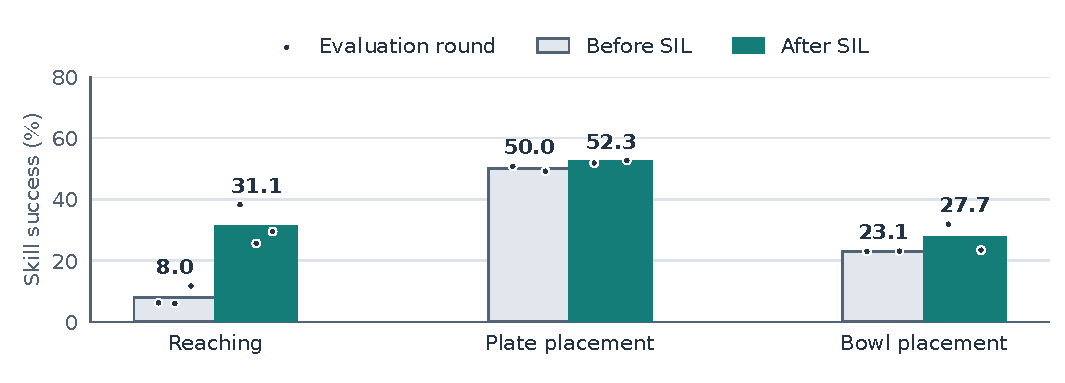
\includegraphics[width=\columnwidth]{figures/skill_retention.pdf}
\caption{Base-policy skill recovery before full-task composition. Bars show means and points show individual evaluation rounds: three for reaching and two for each placement skill, per condition. Reaching uses the instruction \emph{move to \textless object\textgreater}; placement starts with the object already held. Reaching partially recovers while both placement means increase.}
\label{fig:retention}
\end{figure}

Recovery is partial, with placement performance retained while reaching improves. These measurements cover approach and placement. They do not isolate the contribution of self-imitation to final full-task success, and no unbalanced-replay control was run.


\subsection{Auxiliary Study: Intermediate Feedback on LIBERO-Spatial}\label{sec:libero_results}
This study examines one question in isolation: whether intermediate feedback helps full-task RL. It uses a different backbone and does not run the adaptation schedule. It also does not test the milestone credit rule of Section~\ref{sec:composition}.

We fine-tune an OpenVLA-OFT policy with LoRA on complete instructions for the ten LIBERO-Spatial tasks~\cite{openvlaoft,libero}, using our own implementation of SimpleVLA-RL~\cite{simplevlarl}. The terminal-only row is our run under this study's budget, not a result from the SimpleVLA-RL publication. All runs start from one shared checkpoint with 61.0\% success; their final rates are measured after training. Each endpoint uses 300 validation rollouts from one training seed. The dense-plus-phase and terminal-only runs share terminal verifier coefficient 5 and 160 updates. The phase-only run differs in terminal coefficient (1), phase weight, and budget (110 updates), so we report it as a separate configuration rather than as a matched ablation. Dynamic sampling can make equal update counts consume different numbers of rollouts. Environment interactions and GPU-hours per run were not retained, so we compare runs only by updates.

From the shared 61.0\% initial policy, dense-plus-phase feedback reaches 65.3\% after 160 updates, against 61.7\% for terminal-only reward (Table~\ref{tab:libero}). With 300 rollouts, each endpoint's 95\% interval spans about $\pm$5.5 points, so the 3.6-point difference is not resolved by this single-seed comparison. Phase-only feedback reaches 62.3\% under its separate configuration.

These results motivate, but do not establish, the reward choice in the adaptation schedule. The schedule uses binary milestones during full-task learning because a completion predicate is simpler to specify than a continuous progress function for every phase of a new task (Section~\ref{sec:dense_method}). The LIBERO data do not show that binary milestones outperform dense-plus-phase feedback.
\begin{table}[!ht]
\caption{LIBERO-Spatial feedback study (our runs, one seed each). All runs start from a shared 61.0\% policy; endpoints use 300 validation rollouts. CI: Wilson 95\% interval.}
\label{tab:libero}\centering\small
\setlength{\tabcolsep}{4pt}
\begin{tabular}{@{}lrrrr@{}}\toprule
Configuration & Upd. & Final & CI & $\Delta$\\\midrule
Initial policy & 0 & 61.0 & n.r.$^c$ & ---\\
Terminal only$^a$ & 160 & 61.7 & 56.1--67.0 & +0.7\\
Dense + phase & 160 & 65.3 & 59.8--70.5 & +4.3\\
Phase-only$^b$ & 110 & 62.3 & 56.7--67.6 & +1.3\\
\bottomrule
\end{tabular}\\[2pt]
\raggedright\footnotesize$^a$Our implementation of SimpleVLA-RL~\cite{simplevlarl}. $^b$Terminal coefficient 1 instead of 5; not a matched ablation. $^c$Rollout count not recorded. $\Delta$: change from the initial policy, in points.
\end{table}



\subsection{SmolVLA: Complete-Task Adaptation}\label{sec:cdpr_results}
Strict success requires grasp, held lift, intentional release, and correct placement, without carry slip or wrong-placement events. Each attempt starts with an empty gripper and uses one full-task instruction, without teacher assistance. All attempts, including numerical failures, remain in the denominator.

The reported endpoint is evaluated on the development validation panel used during training: 1,024 attempts, 512 plate and 512 bowl, from a fixed set of 128 scenes that is reused at every reading. The endpoint was not chosen by peak score; it is the final checkpoint of the continuation, and the panel peak (71.09\%) is not used.
The adapted controller completes 723 of 1,024 development validation attempts (70.61\% strict success). A binomial 95\% interval is 67.7--73.3\%. Each of the 128 panel scenes contributes eight correlated attempts, so this interval is optimistic. Physical grasp occurs in 92.48\% of attempts and held lift in 88.28\%. Completion rates are 393/512 (76.76\%) for plates and 330/512 (64.45\%) for bowls. Carry slips (16.70\%) and wrong placements (14.16\%) remain the main failure modes.

The most recent evaluation off this panel used the checkpoint after 40M continuation actions. On 512 scenes outside the panel, each repeated four times, it completed 1,258 of 2,048 attempts (61.43\%), against 1,056/2,048 (51.56\%) for the 20M checkpoint on the same scenes. A frozen evaluation of the endpoint on untouched scenes remains to be done, so we treat 70.61\% as a development result.


\subsection{Additional Embodiment: WX200}\label{sec:wx200}
An ongoing experiment applies the schedule to the five-DoF WX200 serial manipulator. Its configured pipeline starts again from pretrained SmolVLA with a new residual, in simulation, rather than transferring the CDPR controller. It therefore tests the schedule on another mechanism, not controller transfer. No WX200 simulation or hardware result is reported in this draft. The final account will record failures, interventions, resets, and training-data sources, and will keep simulation and hardware results separate.
% The WX200 placeholder figure (figures/wx200_slots.pdf, or figures/wx200/panel.pdf
% when supplied) is withheld until real apparatus and rollout images exist.

\subsection{Context and Scope of the Evidence}
Table~\ref{tab:context} places the CDPR result next to related pick-and-place and adaptation results. It is contextual, not a benchmark. Robots, objects, resets, horizons, and success criteria differ across rows, and similar task names do not imply the same task distribution. SmolVLA's score gives half credit each for grasp and placement~\cite{smolvla}; the CDPR score counts only complete strict successes. No row supports a claim of superior performance or sample efficiency.

\begin{table}[!t]
\caption{Contextual results across different settings; not a controlled comparison.}
\label{tab:context}\centering\footnotesize
\setlength{\tabcolsep}{2.5pt}
\begin{tabular}{@{}P{1.75cm}P{2.45cm}P{1.45cm}P{1.35cm}r@{}}\toprule
Work & Robot, task & Human target demos & Metric & Result\\\midrule
SmolVLA~\cite{smolvla} & SO100 (real), cube pick-place & 50/task, multitask & Partial credit & 75\%\\
SimpleVLA-RL~\cite{simplevlarl} & LIBERO-Spatial (sim.) & 1/task & Binary & 98.2\%\\
RL boot.~\cite{nurtdinov2026rlboot} & CDPR (sim.), move to object & 0 & Strict binary & 9.75\%\\
Ours & CDPR (sim.), put into plate/bowl & 0$^a$ & Strict binary & 70.61\%$^b$\\\bottomrule
\end{tabular}\\[2pt]
\raggedright\footnotesize$^a$Automatically generated supervised data in the lineage (Table~\ref{tab:lineage}). $^b$Development panel; off-panel 61.43\% at 40M continuation actions.
\end{table}

The evidence supports a feasibility claim: a pretrained VLA with a newly initialized residual reached 70.61\% strict full-task success on a simulated CDPR, with no human demonstrations collected on that robot. It does not attribute that result to any single stage. Three controls are still missing. The first is direct full-task RL from the same pretrained initialization and residual architecture, with the same information, evaluation, and total interaction budget, including the schedule's acquisition, consolidation-data, and composition interactions and its oracle and assisted data. The second compares protected with unprotected milestone credit from the same consolidated checkpoint. The third compares instruction-balanced with ordinary successful replay under the same data and optimization budget.

The result comes from one training lineage, so no training-seed variation is measured. The development panel was inspected during training, and a frozen evaluation on untouched scenes, with per-episode outcomes, is pending. We also have not tested whether the controller selects objects and destinations from language within a fixed scene. The LIBERO study shares neither the backbone nor the full schedule with the CDPR pipeline. Avoiding human demonstrations does not remove the engineering of simulator, rewards, resets, success predicates, oracle, and assisted controllers, nor the RL compute.


\section{Conclusion}\label{sec:conclusion}
We presented a staged method for adapting a pretrained VLA to a new robot without collecting human demonstrations on that robot. A newly initialized residual over the retained SmolVLA expert acquires component skills through dense-reward RL; self-imitation consolidates them; milestone-based RL learns the complete instruction. On a simulated CDPR the controller reached 70.61\% strict full-task success on a development panel and 61.43\% off-panel at an earlier checkpoint, with automatically generated supervised data in its lineage. Next, we will compare the schedule with budget-matched direct full-task RL from the same initialization, evaluate the frozen controller on untouched scenes, repeat training across seeds, test same-scene instruction changes, and complete the WX200 evaluation.

\bibliographystyle{IEEEtran}
\bibliography{references}
\end{document}
